

\subsection{Chromatic homotopy theory}
\label{ch0:ssec:chromatic-homotopy-theory}

In the abstract we mentioned that the overarching goal of the thesis is to understand aspects of monochromatic homotopy theory. To do this we first need to situate ourselves into the chromatic viewpoint of stable homotopy theory; our approach is inspired by \cite{barthel-beaudry_19}, and will particularly try to tie it to the ideas already introduced. 

In very crude words one can describe chromatic homotopy theory as a reductionist perspective---or maybe a toolbox---for studying the $\infty$-category of spectra, $\Sp$, in which one decomposes it to its smallest fundamental pieces. An often repeated analogy is that of a prism. If $\Sp$ consists of white light, then shining it through the ``chromatic lens'' decomposes it to distinct colors, labeled by a non-negative integer $n$ called the \emph{chromatic height}, analogous to the wavelength of a light wave. 

\begin{center}
\tikzset{every picture/.style={line width=0.75pt}} %set default line width to 0.75pt   

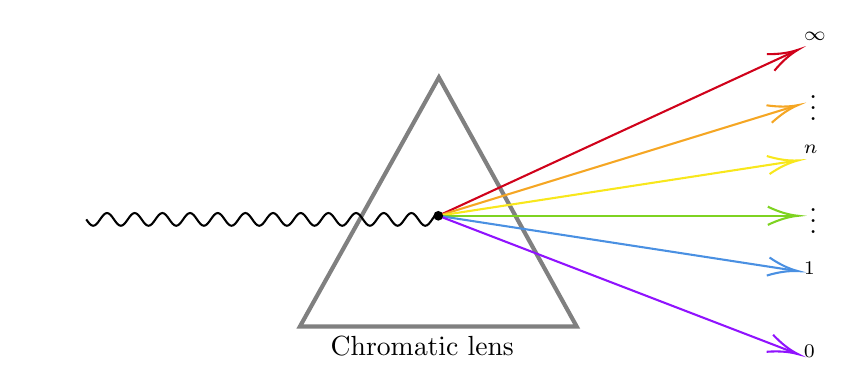
\begin{tikzpicture}[x=1pt,y=1pt,yscale=-1,xscale=1]
    %uncomment if require: \path (0,300); %set diagram left start at 0, and has height of 300
    
%Shape: Triangle [id:dp28924046358844724] 
\draw  [color={rgb, 255:red, 128; green, 128; blue, 128 }  ,draw opacity=1 ][line width=1.5]  (320.22,100) -- (370,190) -- (270,190) -- cycle ;
    %Shape: Wave [id:dp4206352155629708] 
    \draw   (192.8,151.3) .. controls (193.62,152.48) and (194.4,153.6) .. (195.3,153.6) .. controls (196.2,153.6) and (196.98,152.48) .. (197.8,151.3) .. controls (198.62,150.12) and (199.4,149) .. (200.3,149) .. controls (201.2,149) and (201.98,150.12) .. (202.8,151.3) .. controls (203.62,152.48) and (204.4,153.6) .. (205.3,153.6) .. controls (206.2,153.6) and (206.98,152.48) .. (207.8,151.3) .. controls (208.62,150.12) and (209.4,149) .. (210.3,149) .. controls (211.2,149) and (211.98,150.12) .. (212.8,151.3) .. controls (213.62,152.48) and (214.4,153.6) .. (215.3,153.6) .. controls (216.2,153.6) and (216.98,152.48) .. (217.8,151.3) .. controls (218.62,150.12) and (219.4,149) .. (220.3,149) .. controls (221.2,149) and (221.98,150.12) .. (222.8,151.3) .. controls (223.62,152.48) and (224.4,153.6) .. (225.3,153.6) .. controls (226.2,153.6) and (226.98,152.48) .. (227.8,151.3) .. controls (228.62,150.12) and (229.4,149) .. (230.3,149) .. controls (231.2,149) and (231.98,150.12) .. (232.8,151.3) .. controls (233.62,152.48) and (234.4,153.6) .. (235.3,153.6) .. controls (236.2,153.6) and (236.98,152.48) .. (237.8,151.3) .. controls (238.62,150.12) and (239.4,149) .. (240.3,149) .. controls (241.2,149) and (241.98,150.12) .. (242.8,151.3) .. controls (243.62,152.48) and (244.4,153.6) .. (245.3,153.6) .. controls (246.2,153.6) and (246.98,152.48) .. (247.8,151.3) .. controls (248.62,150.12) and (249.4,149) .. (250.3,149) .. controls (251.2,149) and (251.98,150.12) .. (252.8,151.3) .. controls (253.62,152.48) and (254.4,153.6) .. (255.3,153.6) .. controls (256.2,153.6) and (256.98,152.48) .. (257.8,151.3) .. controls (258.62,150.12) and (259.4,149) .. (260.3,149) .. controls (261.2,149) and (261.98,150.12) .. (262.8,151.3) .. controls (263.62,152.48) and (264.4,153.6) .. (265.3,153.6) .. controls (266.2,153.6) and (266.98,152.48) .. (267.8,151.3) .. controls (268.62,150.12) and (269.4,149) .. (270.3,149) .. controls (271.2,149) and (271.98,150.12) .. (272.8,151.3) .. controls (273.62,152.48) and (274.4,153.6) .. (275.3,153.6) .. controls (276.2,153.6) and (276.98,152.48) .. (277.8,151.3) .. controls (278.62,150.12) and (279.4,149) .. (280.3,149) .. controls (281.2,149) and (281.98,150.12) .. (282.8,151.3) .. controls (283.62,152.48) and (284.4,153.6) .. (285.3,153.6) .. controls (286.2,153.6) and (286.98,152.48) .. (287.8,151.3) .. controls (288.62,150.12) and (289.4,149) .. (290.3,149) .. controls (291.2,149) and (291.98,150.12) .. (292.8,151.3) .. controls (293.62,152.48) and (294.4,153.6) .. (295.3,153.6) .. controls (296.2,153.6) and (296.98,152.48) .. (297.8,151.3) .. controls (298.62,150.12) and (299.4,149) .. (300.3,149) .. controls (301.2,149) and (301.98,150.12) .. (302.8,151.3) .. controls (303.62,152.48) and (304.4,153.6) .. (305.3,153.6) .. controls (306.2,153.6) and (306.98,152.48) .. (307.8,151.3) .. controls (308.62,150.12) and (309.4,149) .. (310.3,149) .. controls (311.2,149) and (311.98,150.12) .. (312.8,151.3) .. controls (313.62,152.48) and (314.4,153.6) .. (315.3,153.6) .. controls (316.2,153.6) and (316.98,152.48) .. (317.8,151.3) .. controls (318.62,150.12) and (319.4,149) .. (320.3,149) .. controls (320.33,149) and (320.37,149) .. (320.4,149) ;
    %Straight Lines [id:da3725009850844284] 
    \draw [color={rgb, 255:red, 208; green, 2; blue, 27 }  ,draw opacity=1 ]   (320,150) -- (448.18,90.84) ;
    \draw [shift={(450,90)}, rotate = 155.22] [color={rgb, 255:red, 208; green, 2; blue, 27 }  ,draw opacity=1 ][line width=0.75]    (10.93,-3.29) .. controls (6.95,-1.4) and (3.31,-0.3) .. (0,0) .. controls (3.31,0.3) and (6.95,1.4) .. (10.93,3.29)   ;
    %Straight Lines [id:da04393101077336736] 
    \draw [color={rgb, 255:red, 245; green, 166; blue, 35 }  ,draw opacity=1 ]   (320,150) -- (448.09,110.59) ;
    \draw [shift={(450,110)}, rotate = 162.9] [color={rgb, 255:red, 245; green, 166; blue, 35 }  ,draw opacity=1 ][line width=0.75]    (10.93,-3.29) .. controls (6.95,-1.4) and (3.31,-0.3) .. (0,0) .. controls (3.31,0.3) and (6.95,1.4) .. (10.93,3.29)   ;
    %Straight Lines [id:da6751899671862938] 
    \draw [color={rgb, 255:red, 248; green, 231; blue, 28 }  ,draw opacity=1 ]   (320,150) -- (448.02,130.3) ;
    \draw [shift={(450,130)}, rotate = 171.25] [color={rgb, 255:red, 248; green, 231; blue, 28 }  ,draw opacity=1 ][line width=0.75]    (10.93,-3.29) .. controls (6.95,-1.4) and (3.31,-0.3) .. (0,0) .. controls (3.31,0.3) and (6.95,1.4) .. (10.93,3.29)   ;
    %Straight Lines [id:da7243327342564972] 
    \draw [color={rgb, 255:red, 126; green, 211; blue, 33 }  ,draw opacity=1 ]   (320,150) -- (448,150) ;
    \draw [shift={(450,150)}, rotate = 180] [color={rgb, 255:red, 126; green, 211; blue, 33 }  ,draw opacity=1 ][line width=0.75]    (10.93,-3.29) .. controls (6.95,-1.4) and (3.31,-0.3) .. (0,0) .. controls (3.31,0.3) and (6.95,1.4) .. (10.93,3.29)   ;
    %Straight Lines [id:da7878005985339279] 
    \draw [color={rgb, 255:red, 74; green, 144; blue, 226 }  ,draw opacity=1 ]   (320,150) -- (448.02,169.7) ;
    \draw [shift={(450,170)}, rotate = 188.75] [color={rgb, 255:red, 74; green, 144; blue, 226 }  ,draw opacity=1 ][line width=0.75]    (10.93,-3.29) .. controls (6.95,-1.4) and (3.31,-0.3) .. (0,0) .. controls (3.31,0.3) and (6.95,1.4) .. (10.93,3.29)   ;
    %Straight Lines [id:da4893685373249388] 
    \draw [color={rgb, 255:red, 144; green, 19; blue, 254 }  ,draw opacity=1 ]   (320,150) -- (448.13,199.28) ;
    \draw [shift={(450,200)}, rotate = 201.04] [color={rgb, 255:red, 144; green, 19; blue, 254 }  ,draw opacity=1 ][line width=0.75]    (10.93,-3.29) .. controls (6.95,-1.4) and (3.31,-0.3) .. (0,0) .. controls (3.31,0.3) and (6.95,1.4) .. (10.93,3.29)   ;
    %Straight Lines [id:da9572748849226034] 
    \draw    (320,150) ;
    \draw [shift={(320,150)}, rotate = 0] [color={rgb, 255:red, 0; green, 0; blue, 0 }  ][fill={rgb, 255:red, 0; green, 0; blue, 0 }  ][line width=0.75]      (0, 0) circle [x radius= 1.34, y radius= 1.34]   ;
    
    % Text Node
    \draw (280,192.4) node [anchor=north west][inner sep=0.75pt]   [align=left] {Chromatic lens};
    % Text Node
    \draw (172,145) node [anchor=north west][inner sep=0.75pt]    {$\Sp$};
    % Text Node
    \draw (451,195.4) node [anchor=north west][inner sep=0.75pt]    {$\C_{0}$};
    % Text Node
    \draw (451,82.4) node [anchor=north west][inner sep=0.75pt]    {$\C_{\infty }$};
    % Text Node
    \draw (451,165.4) node [anchor=north west][inner sep=0.75pt]    {$\C_{1}$};
    % Text Node
    \draw (451,123.4) node [anchor=north west][inner sep=0.75pt]    {$\C_{n}$};
    % Text Node
    \draw (453,99.4) node [anchor=north west][inner sep=0.75pt]    {$\vdots $};
    % Text Node
    \draw (453,140.4) node [anchor=north west][inner sep=0.75pt]    {$\vdots $};
    
    
    \end{tikzpicture}
\end{center}

The key to this perspective is that the individual pieces of information can be reassembled back to give information about $\Sp$. This happens in the form of a filtration on the sphere spectrum $\S$, called the \emph{chromatic filtration}. The colimit of this filtration recovers the sphere, hence we can think of the main idea of chromatic homotopy theory as the following: in order to understand $\Sp$, it should be enough to understand the ``chromatic pieces'' individually. 

\begin{remark}
    \label{ch0:rm:quillen-formal-groups}
    Historically these chromatic pieces came about from the relationship between spectra and the algebraic geometry of formal groups, as studied by Quillen in his seminal paper \cite{quillen_1969}. To any complex oriented ring spectrum $E$, one can associate to it a formal group, see for example \cite[Appendix 2]{ravenel_86}. Quillen proved that the formal group associated to the complex cobordism spectrum $\MU$ is the universal formal group over the Lazard ring. The moduli stack of formal groups has a filtration by the \emph{height} of a formal group, and pulling back this filtration to spectra gives precisely the chromatic filtration hinted to above. 
\end{remark}

\subsubsection{Fracture squares and field objects}
\label{ch0:sssec:fracture-squares}

In light of Waldhausen's viewpoint of stable homotopy theory as an enhancement of algebra, usually called \emph{brave new algebra}, one should view the category of spectra $\Sp$ as a homotopical enrichment of the derived category of abelian groups $\Der(\Z)$. We have seen earlier that abelian groups can be studied one prime at the time, which corresponds to studying $\Der(\Z_{(p)})$, the $p$-local derived category. We also want to do this in spectra. 

In \cite{bousfield_1979_localization} Bousfield developed a general machinery for studying localizations on $\Sp$, by inverting maps that are equivalences after tensoring with some spectrum $F$, now called \emph{Bousfield localizations}. The corresponding localization functor is usually denoted $L_F$. 

\begin{example}
    \index{p-localization}
    We can create a version of $p$-localization on $\Sp$, by Bousfield localizing at the $p$-local Moore spectrum $M\Z_{(p)}$, giving a functor usually written 
    \[L_{(p)} \:\Sp \to \Sp_{(p)}.\] 
    On homotopy groups this has the effect of $p$-localizing, in the sense that 
    \[\pi_* L_{(p)}X \simeq \pi_* X [S^{-1}]\simeq \pi_* X \otimes \Z_{(p)}\]
    where $S$ is the set of all primes $q\neq p$. The category of $p$-local spectra, denoted $\Sp_{(p)}$, should then be thought of as a homotopical enrichment of $\Der(\Z_{(p)})$. Just as in \cref{ch0:ex:p-localization-ab-smashing}, the $p$-localization functor $L_{(p)}$ is a smashing localization. 
\end{example}


% \begin{construction}
%     \label{const:bousfield-localization}
%     Let $F$ be a spectrum and $f\colon X\longrightarrow Y$ a map of spectra. We say $f$ is an {\defn $F$-equivalence}, if $f\otimes F$ is an equivalence. If the unique map $0\longrightarrow X$ is an $F$-equivalence, we say $X$ is {\defn $F$-acyclic}. The collection of $F$-acyclic spectra form a localizing ideal (\cref{def:localizing-ideal}), hence the fully faithful inclusion of its left orthogonal complement (\cref{def:left-orthogonal-complement}), denoted {\defn $\sp_F$}, has a left adjoint {\defn $L_F$} as in \cref{ex:localization-from-localizing-subcategory}. This is called the Bousfield localization at $F$, of sometimes just the {\defn $F$-localization}. 
% \end{construction}


%Via the lens of tensor-triangulated geometry, one could think of $\sp$ as the category of quasi-coherent sheaves of tensor-triangulated categories over the Balmer spectrum $\mathrm{Spc}(\sp)$, and similarily for $D(\Z)$. On a spectrum $X$, $p$-localization is given by restricting the corresponding sheaf to the subspectrum lying under the closed point corresponding to $p$. Similarily, for $D(\Z)$: its balmer spectrum is homeomorphic to $\mathrm{Spec}(\Z)$, and localization is restriction to the closed(?) set containing only $p$ and the generic point.


By using the classical arithmetic fracture square, 
\begin{center}
    \begin{tikzcd}
        \Z_{(p)} \arrow[r] \arrow[d] & \Z_p \arrow[d]  \\
        \Q \arrow[r]           & \Q\otimes \Z_p
    \end{tikzcd}
\end{center}

% \begin{center}
%     \begin{tikzpicture}
%         \node (1) {$\Z_{(p)}$};
%         \node (3) [below of=1] {$\Q$};
%         \node (2) [node distance=4cm, right of=1] {$\Z_p$};
%         \node (4) [below of=2] {$\Q\otimes \Z_p$};
%         \draw [-to] (1) -- (2);
%         \draw [-to] (1) -- (3);
%         \draw [-to] (2) -- (4);
%         \draw [-to] (3) -- (4);
%     \end{tikzpicture}
% \end{center}


we see that we can decompose the $p$-local integers into a rational part and a $p$-complete part. This also extends to a general chain complex $A\in \Der(\Z)_{(p)}$, where we have a homotopy pullback square 
\begin{center}
    \begin{tikzcd}
        A \arrow[r] \arrow[d] & A^\wedge_p \arrow[d]  \\
        \Q\otimes A \arrow[r] & \Q\otimes_\Z A^\wedge_p
    \end{tikzcd}    
\end{center}
where $A_p^\wedge$ denotes derived $p$-completion of $A$, as in \cref{ch0:ex:derived-p-completion}. We want to use this to decompose $\Der(\Z_{(p)})$ even further; reduce it to its ``atomic pieces''. This is done via its minimal localizing subcategories. 

\begin{definition}
    \label{ch0:def:minimal-localizing-subcategory}
    \index{Localizing subcategory!Minimal}
    A localizing subcategory $\L\subseteq \C$ is said to be \emph{minimal} if any proper localizing subcategory $\L'\subset \L$ is $(0)$.  
\end{definition}

\begin{remark}
    If $\L$ is a minimal localizing subcategory, then any non-zero object $K\in \L$ generates $\L$ as a localizing subcategory: $\Loc_\C(K)\simeq \L$.
\end{remark}

The study of minimal localizing subcategories is tightly connected to local duality, as in \cref{ch0:ssec:local-duality}. By \cite[2.26]{barthel-heard-valenzuela_2018}, we get from any local duality diagram a fracture square, which for the local duality context $(\Der(\Z_{(p)}), \F_p)$ gives precisely the classical arithmetic fracture square above. 

\begin{proposition}
    Let $\L$ be a minimal localizing subcategory of $\Der(\Z_{(p)})$. Then either $\L \simeq \Der(\Q)$ or $\L$ is equivalent to the category of derived $p$-complete objects, $\L\simeq \Der(\Z_{(p)})^{p-\mathrm{comp}}$.
\end{proposition}

Now, if $\Sp_{(p)}$ is supposed to be a homotopical enrichment of $\Der(\Z_{(p)})$, we should expect there to be an analogy of this decomposition for $p$-local spectra, which is indeed the case. The first to study such squares in topology was Sullivan in his 1970 MIT notes, where he constructed the analogous square for nilpotent spaces, see \cite[3.20]{sullivan_05}. This was later lifted up to spectra by Bousfield in \cite[2.9]{bousfield_1979_localization}, and takes the following form. 

If $\S_{(p)}$ denotes the $p$-local sphere spectrum, we have a spectral arithmetic fracture square\index{Arithmetic fracture square}

\begin{center}
    \begin{tikzcd}
        \S_{(p)} \arrow[r] \arrow[d] & \S_p^\wedge \arrow[d]  \\
        H\Q \arrow[r]           & H\Q\otimes \S_p^\wedge
    \end{tikzcd}
\end{center}

where $\S_p^\wedge$ denotes the $p$-complete sphere. This also extends to any object $X\in \Sp_{(p)}$, just like for $A\in \Der(\Z_{(p)})$. 

We can then ask the natural question: do these give all the minimal localizing subcategories of $\Sp_{(p)}$? This was indeed the case for $\Der(\Z_{(p)})$, but now, in the more complicated world of spectra, this is no longer true. We now have an infinite sequence of minimal localizing subcategories, indexed by a non-negative integer $n$, that ``interpolates'' between the two minimal localizing subcategories of $\Der(\Z_{(p)})$. 

\begin{remark}
    In fact, even more is true: By the failure of the telescope conjecture, see \cite{burklund-hahn-levy-schlank_23}, there are at least two such infinite sequences. We can make sure that there is a single such sequence if we translate over to compactly generated $\otimes$-ideals, but for the above exposition, we have chosen to sweep these details under a big old telescope-shaped rug.
\end{remark}

We can identify these ``intermediary'' subcategories by an analysis of field objects. For $\Der(\Z_{(p)})$ there are exactly two field objects associated to the unit $\Z_{(p)}$, namely $\Q$ and $\F_p$; each is obtained by either killing or inverting $p$. 

For $\Sp_{(p)}$ we have a field object for any number $n\in \N\cup \{\infty\}$, which we denote by $\Kpn$. We have $K_p(0)=H\Q$ and $K_p(\infty) = H\F_p$, showing that this sequence of field objects really forms an interpolation between the two field objects coming from algebra. 

\begin{notation}
    \index{Morava $K$-theory}
    \index{Spectra!$K_p(n)$-local}
    The object $\Kpn$ is called the \emph{Morava K-theory of height $n$}. The associated category of $\Kpn$-local spectra---meaning the category obtained by Bousfield localization at $\Kpn$---is denoted $\SpKpn$. 
\end{notation}

These field objects $\Kpn$ were constructed by Morava in the early 70's, by topologically interpreting the unique geometric point in the moduli stack of formal groups, determined by the height $n$ Honda formal group; the categories of $\Kpn$-local spectra have been under intense study ever since. We do not cover precise constructions here and instead refer the interested reader to \cite{hovey-strickland_99}. The Morava $K$-theory spectrum $\Kpn$ is, however, uniquely determined by the following properties. 

\begin{proposition}
    \label{ch0:prop:properties-of-K(n)}
    Let $p$ be a prime and $n$ a non-negative integer. The height $n$ Morava K-theory spectrum $\Kpn$ is a complex oriented $\E_1$-ring spectrum with coefficients 
    \[\Kpn_*:=\pi_* \Kpn \simeq \F_p[v_n^{\pm}],\]
    with $|v_n|=2p^n-2$, whose associated formal group is the height $n$ Honda formal group. Furthermore, for any two spectra $X$ and $Y$, there is a Künneth isomorphism 
    \[\Kpn_*(X\times Y)\simeq \Kpn_*X\otimes_{\Kpn_*} \Kpn_*Y.\]
\end{proposition}

\begin{remark}
    By \cite[7.5]{hovey-strickland_99} the categories of $\Kpn$-local spectra are minimal. One can show that for finite heights $n$, the categories $\Sp_\Kpn$ are all the minimal localizing subcategories of $\Sp_{(p)}$. But, there are some issues with height $\infty$, not yet allowing us to create a full classification. 
\end{remark}

\begin{remark}
    While the $\E_1$-ring structure on $\Kpn$ can be shown to be essentially unique, it does admit uncountably many $\E_1$-$\MU$-algebra structures---see \cite{angeltveit_2011}. 
\end{remark}

\begin{remark}
    \label{ch0:rm:SpKn-not-rigidly-generated}
    The category $\Sp_\Kpn$ is compactly generated by dualizable objects, but it is \emph{not} a rigidly compactly generated category, in the sense of \cref{ch0:rigidly-generated-category}, as the unit $L_{\Kpn}\S$---the $\Kpn$-local sphere---is not compact.  
\end{remark}

It now remains to understand how these field objects $\Kpn$ are related to the spectral arithmetic fracture square above. If the $\Sp_\Kpn$'s all form minimal localizing subcategories, and they in some sense interpolate between rational information at height $0$, and $p$-local information at height $\infty$, then we should perhaps expect there to be an infinite sequence of fracture squares---starting from $L_\Q \S \simeq H\Q$, and converging to $\S_{(p)}$. This is indeed the case. 

\begin{construction}
    \label{ch0:const:chromatic-fracture-square}
    Let $L\np := L_{K_p(0)\vee \cdots \vee \Kpn}$. By Ravenel's smash product theorem, see \cite[7.5.6]{ravenel_92}, the functor $L\np\colon \Sp_{(p)}\longrightarrow \Sp_{(p)}$ is a smashing localization. The \emph{chromatic fracture square}\index{Chromatic fracture square}, generally attributed to Hopkins, is then of the form 
    \begin{center}
        \begin{tikzcd}
            L\np\S \arrow[r] \arrow[d] & L_{\Kpn}\S \arrow[d]  \\
            L_{n-1,p}\S \arrow[r] & L_{n-1,p}\S\otimes L_{\Kpn}\S 
        \end{tikzcd}    
    \end{center}
    By definition we have $L_{0,p} \S = L_\Q \S \simeq H\Q$, hence the starting point is exactly what we wanted. As alluded to earlier, the spectra $L\np\S$ assemble into a a filtration, 
    \[\cdots \longrightarrow L_{3,p}\S \longrightarrow L_{2,p}\S \longrightarrow L_{1,p}\S \longrightarrow L_{0,p} \S = L_\Q\S\]
    called the chromatic filtration. By the chromatic convergence theorem of Hopkins-Ravenel, see \cite[7.5.7]{ravenel_92}, we can recover $\S_{(p)}$ as the colimit of this diagram. This is the more precise meaning of the statement that the Morava $K$-theory spectra $\Kpn$ allow us to interpolate between rational and $p$-local information. 
\end{construction}

\begin{remark}
    \label{ch0:rm:chromatic-square-from-duality}
    The arithmetic fracture square for $\Der(\Z_{(p)})$ was ``categorified'' into the local duality diagram for the local duality context $(\Der(\Z_{(p)}), \F_p)$, in the sense that the associated fracture square to the diagram was exactly the arithmetic one. We would like to have a similar property for the chromatic fracture square. In order to do this, we first need to understand the localization functor $L\np$ that showed up above. 
\end{remark}  






\subsubsection{Morava \texorpdfstring{$E$}{E}-theories}
\label{ch0:sssec:morava-E-theories}

In the previous section, we obtained a localization functor $L\np$, which collected the chromatic information from height $0$ up to and including height $n$. This localization is good for many purposes, but when we later want to tie the homotopy theory to algebra, we need another approach. In particular, we want a spectrum $E$ such that the Bousfield localization $L_E$ is the same as $L\np$. There are several approaches to obtaining such a spectrum $E$, and the goal of this section is to give a brief overview of the ones we will need later. We will assume general knowledge about formal groups---all needed background can be found in \cite[Appendix 2]{ravenel_86}. Our overview is inspired by lecture notes made by Rognes, \cite{rognes_2023}. 

The first construction of a spectrum $E$ satisfying the above is due to Morava, and is based on the aforementioned connection between complex oriented cohomology theories and formal groups. In honor of this one usually refers to any conveniently nice spectrum with the property that $L_E \simeq L\np$ as \emph{Morava $E$-theory}\index{Morava $E$-theory}.

\begin{construction}
    \index{Lubin--Tate ring}
    Let $p$ be a prime and $\kappa$ a perfect field of characteristic $p$. Lubin and Tate proved in \cite{lubin-tate_66} that for any formal group law $F$ of height $n$ over $\kappa$, there is a universal deformation $\bar{F}$ over the ring $E(\kappa, F)=\W(k)[\![ u_1, \ldots, u_{n-1}]\!]$ of formal power series over the Witt vectors of $\kappa$. This ring is now usually called the \emph{Lubin-Tate ring} of $F$. Using the algebraic geometry of formal groups, Morava interpreted this universal deformation as a formal neighborhood of the height $n$ Honda formal group law $H_n$, and via a topological realization process obtained a spectrum $E^{Mor}\np$.
\end{construction}

We will not explain in detail how Morava obtained such a spectrum, and instead cover a more simple approach, yielding a slightly different spectrum. This spectrum was originally constructed by Johnson and Wilson in \cite{johnson-wilson_75}, by using the theory of manifolds with singularities developed by Baas-Sullivan (see \cite{baas_73a} and \cite{baas_73b}). We take a more modern approach, utilizing Brown representability. 

\begin{construction}
    \index{Johnson--Wilson theory}
    Let $p$ be a prime, $n$ a non-negative integer and denote by $E_p(n)_*$ the graded ring $\Z_{(p)}[v_1, \ldots, v_{n-1}, v_n^{\pm}]$, where $|v_i| = 2p^i-2$. This is obtained from the coefficient ring of the Brown--Peterson spectrum $\BP$---essentially a $p$-local version of the complex cobordism spectrum $\MU$---by killing all the generators $v_k$ for $k>n$ and inverting $v_n$. This ring is a $\BP_*$-module, and satisfies a certain flatness condition called \emph{Landweber flatness}, see \cite{landweber_76}; tensoring with $E_p(n)_*$ is not exact as a $\Mod_{\BP_*}\to \Mod_{E_p(n)_*}$, but it \emph{is} exact as a functor on $\Comod_{\BP_*\BP}$. Hence, as $\BP$-homology lands in this Grothendieck abelian category, we can define a functor 
    \[\Sp \overset{\BP_*}\to \Comod_{\BP_*\BP}\overset{E_p(n)_*\otimes_{\BP_*}-}\to \mathrm{gr}\Ab,\]
    which by the properties mentioned is a homology theory. Via Brown's representability theorem, see \cite[Theorem 1]{brown_1962}, this homology theory is governed by a spectrum $E_p(n)$ such that $\pi_* E_p(n) \simeq E_p(n)_*$. This spectrum is called the height $n$ \emph{Johnson-Wilson theory}. 
\end{construction}

\begin{remark}
    \label{ch0:rm:K-as-quotient-of-E}
    The ring $E_p(n)_*$ is local, and hence has a unique maximal ideal $I_n = (p, v_1, \ldots, v_{n-1})$ called the Landweber ideal. The quotient of $E_p(n)_*$ by this maximal ideal gives $E_p(n)_*/I_n \cong \F_p[v_n^{\pm}] = \Kpn_*$. %By utilizing some results from \cite{ekmm_2007}, this can also be suitably interpreted as a quotient of spectra. 
\end{remark}

\begin{definition}
    An $\E_1$-ring spectrum $R$ is said to be concentrated in degrees divisible by $q$ if $\pi_k R \cong 0$ for all $k \not = 0 \mod q$. 
\end{definition}

\begin{proposition}
    \label{ch0:prop:Johnson-Wilson-properties}
    If $p$ is a prime and $n$ a non-negative integer, then the associated height $n$ Johnson--Wilson theory $E_p(n)$ is a complex oriented, Landweber exact $\E_1$-ring spectrum, concentrated in degrees divisible by $2p-2$. 
\end{proposition}

\begin{remark}
    The Johnson--Wilson spectrum $E_p(n)$ is also periodic, with period $2p^n-2$. This is the same periodicity as the Morava $K$-theory spectrum. 
\end{remark}

Later, using a $2$-periodic analogue of the universal deformation theory of Lubin and Tate, Hopkins and Miller constructed a $2$-periodic $\E_1$-version of Morava's spectrum, which was later enhanced to an $\E_\infty$-ring spectrum $E\np$ via Goerss--Hopkins theory, see \cite{goerss-hopkins_04}, or \cite{pstragowski_vankoughnett_2022} for a modern treatment. In essence, Hopkins and Miller constructed a functor from pairs $(\kappa, F)$ of a perfect field $\kappa$ of characteristic $p$, together with a choice of height $n$ formal group law $F$, to even periodic ring spectra. For a specific choice of $(\kappa, F)$, we can summarize the properties as follows.  

\begin{proposition}
    Let $p$ be a prime, $\kappa$ a perfect field of characteristic $p$, and $F$ a formal group law of height $n$ over $\kappa$. The spectrum $E(\kappa,F)$ is a $2$-periodic, complex oriented, Landweber exact $\E_\infty$-ring spectrum, such that 
    \[\pi_0 E(\kappa,F)=\W(\kappa)[\![ u_1, \ldots, u_{n-1}]\!]\] 
    and the associated formal group law is the universal deformation of $F$. 
\end{proposition}


%Let $FGL$ denote the category of pairs $(k, F)$ for $k$ a perfect field of characteristic $p$ and $F$ a formal group of height $n$ over $k$. Morphisms in the category are pairs $(f,\phi)\colon (k, F)\to (k', F')$ where $f\colon k'\to k$ is a ring homomorphism and $\phi\colon F\to f^* F'$ is an isomorphism.  

%\begin{theorem}[{\cite[2.1]{rezk_98}}]
%    There is a functor $E(-,-)\colon FGL \longrightarrow Alg(\sp)$
%\end{theorem}

\begin{definition}
    \index{Lubin--Tate theory}
    For the specific choice $(\kappa,F) = (\F_{p^n}, H_n)$---here $H_n$ again denotes the height $n$ Honda formal group law---we simply write $E(\F_{p^n}, H_n) = E\np$, and call it the height $n$ \emph{Lubin--Tate theory} at the prime $p$. 
\end{definition}

\begin{remark}
    One can also study maps of ring spectra $E\np \longrightarrow K\np$ such that the induced map on homotopy groups is given by taking the quotient by the maximal ideal, just as in \cref{ch0:rm:K-as-quotient-of-E}. Such spectra $K\np$ are $2$-periodic versions of Morava $K$-theory and have been studied, for example, in \cite{hopkins-lurie_17} and \cite{barthel-pstragowski_2021}. 
\end{remark}

\begin{remark}
    \index{Johnson--Wilson theory!Complete}
    One nice benefit of $E\np$ compared to $E_p(n)$---other than it being fully coherently commutative rather than just $\E_1$---is that the former is $\Kpn$-local, making its chromatic behavior even more interesting. In fact, the unit map $L_{\Kpn}\S \longrightarrow E\np$ is a pro-Galois extension in the sense of \cite{rognes_08}, where the Galois group is the extended Morava stabilizer group $\G_n$, see \cite{devinatz-hopkins_2004}. We can, however, also make the latter $\Kpn$-local, by instead using a completed version $\widehat{E}_p(n)$, often called \emph{completed Johnson-Wilson theory}. It has most of the same properties as that of $E_p(n)$, except that it is $\Kpn$-local and its coefficients are $p$-adic and $I_n$-complete: 
    \[\widehat{E}_p(n)_* \simeq \Z_p[v_1, \cdots, v_{n-1}, v_n^{\pm}]^\wedge_{I_n}.\]
\end{remark}

\begin{remark}
    An $\E_\infty$-version of Morava's original spectrum $E\np^{Mor}$ can be recovered from $E\np$ by taking the homotopy fixed points with respect to the Galois action from $\mathrm{Gal}(\F_{p^n}/\F_p)\cong \Z/n$. Another alternative is to use $E\np^{h\F_p^\times}$. This spectrum is concentrated in degrees divisible by $2p-2$, hence serves as a nice $\E_\infty$-version of the $\E_1$-ring spectrum $E_p(n)$. This is the model of $E$ used, for example, in Barkan's monoidal algebraicity theory, see \cite{barkan_2023}. 
\end{remark}

We have now introduced several versions of Morava $E$-theories, all in light of trying to understand the localization functor $L\np$. Hence, we round off this section by stating that the Bousfield localizations at any of the above $E$-theories are equivalent. 

\begin{proposition}[{\cite[1.12]{hovey_95}}]
    \label{ch0:prop:all-E-local-cats-are-equivalent}
    If $p$ is a prime and $n$ a non-negative integer, then there are symmetric monoidal equivalences of stable $\infty$-categories 
    \[\Sp_{L\np} \simeq \Sp_{E_p(n)} \simeq \Sp_{E(k,F)}\simeq \Sp_{E\np} \simeq \Sp_{\widehat{E}_p(n)}\simeq \Sp_{E\np^{h\F_p^\times}}.\]
    In fact, all of these categories are equivalent as subcategories of $\Sp$. Furthermore, if $E$ is any Landweber exact $v_n$-periodic $\BP$-algebra, then $\Sp_E$ is equivalent to the above categories. 
\end{proposition}

\begin{notation}
    \index{Spectra!$E\np$-local}
    We will use the common notation $\Sp\np$ for any of the above categories. We will call it the category of $E\np$-local spectra, or sometimes the category of height $n$ spectra, or even just the category of $E$-local spectra when the height and prime are understood. 
\end{notation}

\begin{remark}
    \index{Compactly generated!Rigid}
    The category $\Sp\np$ is rigidly compactly generated by the collection of dualizable objects $\{L\np F\}$, where $F$ is a finite spectrum---in stark contrast to $\SpKpn$, see \cref{ch0:rm:SpKn-not-rigidly-generated}. In fact, $\Sp\np$ is rigidly compactly generated by its unit $L\np\S$. 
\end{remark}

\begin{remark}
    Note that even though the different models for $\Sp\np$ are equivalent, some of them have non-equivalent associated module categories. For example, $\Mod_{E\np}\not \simeq \Mod_{E_p(n)}$, as the ring spectra $E\np$ and $E_p(n)$ have different periodicity---the former is $2$-periodic while the latter is $(2p^n-2)$-periodic. Whenever such a distinction is relevant, we will make this explicit. 
\end{remark}





\subsubsection{Monochromatic spectra and local duality}
\label{ch0:sssec:monochromatic-duality}

Recall from \cref{ch0:sssec:fracture-squares} that our goal is to understand the $\Kpn$-local pieces of the category of $p$-local spectra, $\Sp_{(p)}$. By \cref{ch0:rm:chromatic-square-from-duality}, we are looking for a local duality theory that categorifies the chromatic fracture square. In this section, we construct precisely such a local duality theory, both for $\Sp\np$ and for modules over $E$ for some choice of Morava $E$-theory. 



\begin{definition}
    \label{ch0:def:monochromatic-spectrum}
    \index{Monochromatic!spectrum}
    \index{Spectra!Monochromatic}
    A spectrum $X$ is called \emph{$n$-monochromatic} if it is $E\np$-local and $E_{n-1,p}$-acyclic. The full subcategory of $n$-monochromatic spectra will be denoted $\M\np$ and referred to as the height $n$ monochromatic category.
\end{definition}

If the height is understood, we will sometimes drop the $n$ from the notation. We have a convenient way to produce monochromatic spectra from $E\np$-local ones. 

\begin{definition}
    \index{Monochromatic!Layer}
    Let $X\in \sp\np$. The fiber of the localization $X\longrightarrow L_{n-1,p}X$, which we denote $M\np X$ is called the $n$'th \emph{monochromatic layer} of $X$ at the prime $p$.
\end{definition}

\begin{remark}
    \index{Monochromatization}
    If $X$ is a monochromatic spectrum, then it is $L_{n-1,p}$-acyclic by definition, i.e., $L_{n-1,p}X\simeq 0$. Hence the fiber sequence 
    \[M\np X\longrightarrow X\longrightarrow L_{n-1,p}X\]
    gives an equivalence $X\simeq M\np X$. The fully faithful inclusion $\M\np\longrightarrow \Sp\np$ has a right adjoint, given by $X\longmapsto M\np X$, which we call the \emph{monochromatization}. 
\end{remark}

\begin{proposition}
    \label{ch0:prop:monochromatization-is-smashing}
    \index{Localization!Smashing}
    The monochromatization functor 
    \[M\np\colon \sp\np\longrightarrow \M\np\] 
    is a smashing colocalization, in the sense of \cref{ch0:rm:smashing-colocalization}.
\end{proposition}
\begin{proof}
    As far as we are aware, this proposition was first proved in \cite[Sec 6.3]{bousfield_1996} in the case of finite monochromatization, i.e., the fiber functor of the finite localization $L\np^f$. The proof, however, uses the arguments from \cite[2.10]{bousfield_1979_bool}, which also work for the non-finite case. A simplified argument uses Ravenel's smash product theorem, see \cite[7.5.6]{ravenel_92}, stating that the localization $L_{n-1,p} = L_{E_{n-1,p}}$ is smashing. Hence, we can simply compare the two fiber sequences
    \[M\np \S \otimes X \longrightarrow X \longrightarrow L_{n-1,p}\S\otimes X\] 
    and 
    \[M\np X\longrightarrow X\longrightarrow L_{n-1,p} X,\]
    which immediately identifies the fibers.  
\end{proof}


% \begin{proof}
%     One can also argue as follows: As $M_n(-)$ is a right adjoint to a fully faithful inclusion, it is, by definition, a colocalization. As $L_{n-1}$ is a smashing localization the localized unit $L_{n-1}\S_n$ is an idempotent algebra in $\sp\np$, and $L_{n-1}$ is equivalent to $L_{n-1}\S_n\otimes (-)$. Dually, then, the fiber of the unit map $\S_n\longrightarrow L_{n-1}\S_n$, which we denoted by $M_n\S_n$, is then an idempotent coalgebra, and the fiber functor $M_n(-)$ is identified with $M_n\S_n\otimes (-)$. 
% \end{proof}

We are now almost ready to construct local duality for chromatic homotopy theory. The last thing we need is a good set of compact objects to form our local duality context. 

\begin{definition}
    \label{ch0:def:type-n-spectrum}
    \index{Type $n$ spectrum}
    We say a finite $p$-local spectrum $X$ is of \emph{type $n$} if $\Kpn_* X\not\cong 0$ and $K_p(m)_*X\cong 0$ for all $m<n$. 
\end{definition}

As a consequence of the thick subcategory theorem of Hopkins--Smith, \cite[Theorem 7]{hopkins-smith_1998}, such spectra exist for all primes $p$ and non-negative integers $n$. For example, if $n=1$, we can choose the mod $p$ Moore spectrum $\S/p$.  

\begin{construction}
    \label{ch0:const:chromatic-duality}
    \index{Local duality!Diagram}
    Let $n$ be a non-negative integer and $p$ a prime. For a finite type $n$ spectrum $F(n)$, its $L\np$-localization $L\np F(n)$ is a compact object in $\Sp\np$ and hence generates a localizing tensor ideal $\Sp\np\Ktors$, where $\K$ denotes the singleton set $\{L\np F(n)\}$. By \cref{ch0:thm:local-duality}, we have a corresponding local duality diagram for the local duality context $(\Sp\np, \K)$:
    \begin{center}
    \begin{tikzcd}
            & {\sp\np\Kloc} \\
            & {\sp\np} \\
            {\sp\np\Ktors} && {\sp\np\Kcomp}
            \arrow["L", xshift=-2pt, from=2-2, to=1-2]
            \arrow[xshift=2pt, from=1-2, to=2-2]
            \arrow["\Lambda", yshift=2pt, xshift=2pt, from=2-2, to=3-3]
            \arrow[yshift=-2pt, xshift=-1pt, from=3-3, to=2-2]
            \arrow["\Gamma", yshift=-2pt, xshift=2pt, from=2-2, to=3-1]
            \arrow[yshift=2pt, xshift=-1pt, from=3-1, to=2-2]
            \arrow[bend left=35, dashed, from=3-1, to=1-2]
            \arrow[bend left=35, dashed, from=1-2, to=3-3]
            \arrow["\simeq"', swap, from=3-1, to=3-3]
    \end{tikzcd}    
    \end{center}
\end{construction}

We wanted to construct a local duality diagram that categorified the chromatic fracture square\index{Chromatic fracture square}, and we claim that the above diagram does the trick. 

\begin{proposition}
    \label{ch0:prop:torsion-is-monochromatic}
    There are equivalences
    \begin{enumerate}
        \item $\Sp\np\Ktors\simeq \M\np$
        \item $\sp\np\Kloc\simeq \Sp_{n-1,p}$
        \item $\Sp\np\Kcomp\simeq \SpKpn$
    \end{enumerate} 
    of symmetric monoidal stable $\infty$-categories. 
\end{proposition}

\begin{remark}
    These equivalences are by now classical, but we recall an argument for the reader's convenience and for building intuition. 
\end{remark}

\begin{proof}
    By definition the category $\M\np$ is the full subcategory of $L_{n-1,p}$-acyclic objects in $\Sp\np$, and $M\np$ coincides with the $L_{n-1,p}$-acyclification. By \cite[6.10]{hovey-strickland_99} $L_{n-1,p}$-localization is the finite localization away from $L\np F(n)$, which proves equivalence $(2)$. This also means that the $L_{n-1,p}$-acyclic objects are precisely the objects in 
    \[\Loc^\otimes_{\Sp\np}(L\np F(n))=:\Sp\np\Ktors,\]
    giving the equivalences $\M\np \simeq \Sp\np\Ktors$ and $\Gamma \simeq M\np$, proving $(1)$. One can also see this by the fact that $M\np$ preserves compact objects, as it is smashing by \cref{ch0:prop:monochromatization-is-smashing}, which also implies that $\M\np$ is closed under colimits. The compact objects $L\np X\in \Sp\np$ for $X$ any finite spectrum of type $n$ are also monochromatic, as 
    \[E_{n-1,p *} L\np X \cong E_{n-1,p *}X\cong 0,\]
    and they do in fact generate $\M\np$ under colimits. 



    % Notice that if we prove $(1)$, then $(2)$ immediately follows by the definition of being monochromatic. For $(1)$, then, note that as $L_{n-1}$ is smashing, $\M\np$ is closed under colimits. It is also closed under suspension and retracts, and by \cref{prop:monochromatization-is-smashing}, it is closed under tensoring with objects in $\sp\np$. This means that it is a localizing ideal. The object $K=L_n F(n)$ is both $K$-torsion and monochromatic, as it is $E_n$-local by assumption, and $E_{n-1 *} K \cong E_{n-1 *}F(n)\cong 0$. As $M_n$ is smashing by \cref{prop:monochromatization-is-smashing}, it preserves compact objects. Hence, also $K$ is compact in $\M\np$. 
    
    
    % It is, in addition, compact, as we have for all filtered diagrams $\colim_\alpha X_\alpha$ where $X_\alpha\in \M\np$ that
    % \begin{align*}
    %     \map_{\M\np}(K, \colim_\alpha X_\alpha) 
    %     &\simeq \map_{\sp\np}(K, \colim_\alpha X_\alpha) \\
    %     &\simeq \colim_\alpha \map_{\sp\np}(K, X_\alpha) \\ 
    %     &\simeq \colim_\alpha \map_{\M\sp\np}(K, X_\alpha).
    % \end{align*}
    % In particular this means that $\sp\np^{K-tors}\subseteq \M\np$. In fact, the same above sequence of equivalences holds for the $L_n$-localization of any finite spectrum of type $\geq n$. Hence, all these are monochromatic. These spectra also generate $\M\np$ under colimits, . Since all these are $K$-torsion

    The equivalence in $(3)$ follows from \cite[2.34]{barthel-heard-valenzuela_2018}, which shows that $\Lambda_\K$ can be identified with the Bousfield localization $L_K$ whenever the set of compact objects in a local duality context $(\C, \K)$ consists of a single element $\K=\{K\}$. Note that the localization $L_K$ is not the same as the functor $L_\K$. This, together with the fact that the Bousfield localizations $L_\Kpn$ and $L_{L\np F(n)}$ agree by \cite[7.1]{hovey-strickland_99}, proves $(3)$. 
\end{proof}

\begin{remark}
    This means that the equivalence $\Sp\np\Ktors\overset{\simeq}\longrightarrow \Sp\np\Kcomp$ is given by the adjoint pair $(L_{\Kpn}\dashv M\np)$, which recovers the symmetric monoidal equivalence $\M\np \simeq \SpKpn$ of \cite[6.19]{hovey-strickland_99}. 
\end{remark}

\begin{remark}
    \index{Chromatic fracture square}
    The local duality diagram we obtained in \cref{ch0:const:chromatic-duality}, gives via \cite[2.26]{barthel-heard-valenzuela_2018} precisely the chromatic fracture square
    \begin{center}
        \begin{tikzcd}
            L\np\S \arrow[r] \arrow[d] & L_{\Kpn}\S \arrow[d]  \\
            L_{n-1,p}\S \arrow[r] & L_{n-1,p}\S\otimes L_{\Kpn}\S 
        \end{tikzcd}    
    \end{center}
    ---exactly as we wanted in \cref{ch0:rm:chromatic-square-from-duality}.   
\end{remark}

\begin{remark}
    By \cref{ch0:rm:tors-loc-comp-compactly-generated}, all the categories in the local duality diagram are compactly generated. But, the unit $L_{\Kpn}\S$ in $\SpKpn$ is not compact, so by \cref{ch0:rm:compacts-equal-dualizable} the compact and dualizable objects differ. The same is then necessarily true for $\M\np$.
\end{remark}

We have a similar construction in the case of $E$-modules, where $E$ is any of the models for Morava $E$-theory we presented in \cref{ch0:sssec:morava-E-theories}. For simplicity, let us assume $E= E_p(n)$, and recall that we have a unique maximal Landweber ideal $I_n = (p, v_1, \ldots, v_{n-1})\subseteq  \pi_* E$. Using the convention that $p = v_0$ we have for any $i$ a map $v_i \: \Sigma^{2p^i-2} E \to E$; we denote its cofiber by $E/v_i$. Letting $E/I_n = \bigotimes_{i=0}^n E/v_i$ we have the following local duality result---see also \cite{greenlees-may_1995} and \cite[Section 3.1]{barthel-heard-valenzuela_2018} for more details. 

\begin{construction}
    \label{ch0:const:chromatic-duality-modules}
    \index{Johnson--Wilson theory}
    Let $n$ be a non-negative integer, $p$ a prime, and $E$ some height $n$ Morava $E$ theory---for example Johnson--Wilson theory or Lubin--Tate theory. The object $E/I_n$ is compact in $\ModE$ and generates a localizing tensor ideal $\Modt := \Loc^\otimes_{\ModE}(E/I_n)$, where we use the superscript $I_n$ for simplicity. By \cref{ch0:thm:local-duality}, we have a corresponding local duality diagram for the local duality context $(\ModE, E/I_n)$:
    \begin{center}
        \begin{tikzcd}
                & {\ModE\Inl} \\
                & {\ModE} \\
                {\Modt} && {\Modc}
                \arrow["L", xshift=-2pt, from=2-2, to=1-2]
                \arrow[xshift=2pt, from=1-2, to=2-2]
                \arrow["\Lambda", yshift=2pt, xshift=2pt, from=2-2, to=3-3]
                \arrow[yshift=-2pt, xshift=-1pt, from=3-3, to=2-2]
                \arrow["\Gamma", yshift=-2pt, xshift=2pt, from=2-2, to=3-1]
                \arrow[yshift=2pt, xshift=-1pt, from=3-1, to=2-2]
                \arrow[bend left=35, dashed, from=3-1, to=1-2]
                \arrow[bend left=35, dashed, from=1-2, to=3-3]
                \arrow["\simeq"', swap, from=3-1, to=3-3]
        \end{tikzcd}    
    \end{center}
    Just as in \cref{ch0:prop:torsion-is-monochromatic}, there are equivalences 
    \begin{enumerate}
        \item $\ModE\Int \simeq \M\np\ModE$,
        \item $\ModE\Inl \simeq L_{n-1,p}\ModE$ and
        \item $\ModE\Inc \simeq L_{\Kpn}\ModE$,
    \end{enumerate}
    being the full subcategories of monochromatic $E$-modules, $E_{n-1,p}$-local $E$-modules and $\Kpn$-local $E$-modules respectively. 
\end{construction}

